\documentclass[aspectratio=169]{beamer}
\setbeamertemplate{footline}{}
\setbeamertemplate{navigation symbols}{}

% ---------------------------------------------------------
% Nord Color Palette
% ---------------------------------------------------------
\definecolor{Nord0}{HTML}{2E3440} % #2E3440
\definecolor{Nord1}{HTML}{3B4252} % #3B4252
\definecolor{Nord2}{HTML}{434C5E} % #434C5E
\definecolor{Nord3}{HTML}{4C566A} % #4C566A
\definecolor{Nord4}{HTML}{D8DEE9} % #D8DEE9
\definecolor{Nord5}{HTML}{E5E9F0} % #E5E9F0
\definecolor{Nord6}{HTML}{ECEFF4} % #ECEFF4
\definecolor{Nord7}{HTML}{8FBCBB} % #8FBCBB
\definecolor{Nord8}{HTML}{88C0D0} % #88C0D0
\definecolor{Nord9}{HTML}{81A1C1} % #81A1C1
\definecolor{Nord10}{HTML}{5E81AC} % #5E81AC
\definecolor{Nord11}{HTML}{BF616A} % #BF616A
\definecolor{Nord12}{HTML}{D08770} % #D08770
\definecolor{Nord13}{HTML}{EBCB8B} % #EBCB8B
\definecolor{Nord14}{HTML}{A3BE8C} % #A3BE8C
\definecolor{Nord15}{HTML}{B48EAD} % #B48EAD

% ---------------------------------------------------------
% Theme Setup
% ---------------------------------------------------------
\usetheme{default}

% Background + text
\setbeamercolor{background canvas}{bg=Nord0}
\setbeamercolor{normal text}{fg=Nord6}

% Frame titles
\setbeamercolor{frametitle}{bg=Nord0, fg=Nord8}

\setbeamertemplate{frametitle}{%
  \vspace{0.6em}%
  \nointerlineskip%
  \begin{beamercolorbox}[wd=\textwidth, leftskip=-0.1cm, rightskip=0.3cm]{frametitle}%
    % Nord14 triangle pointing right → toward the title text
    \tikz[baseline=-0.23ex]{
      \fill[Nord14] (0,0) -- (0,1.2ex) -- (1.2ex,0.6ex) -- cycle;
    }%
    \hspace{0.6em}%
    {\color{Nord8}\usebeamerfont{frametitle}\insertframetitle}%
    \vspace{0.3em}%
  \end{beamercolorbox}%
}
\setbeamerfont{frametitle}{size=\large,series=\bfseries}

% Table of Contents
% Colors/fonts for ToC entries

% Colors + fonts
% Slightly larger section text
\setbeamerfont{section in toc}{size=\large}
\setbeamerfont{subsection in toc}{size=\normalsize}

% Soft Nord colors
\setbeamercolor{section in toc}{fg=Nord6}
\setbeamercolor{subsection in toc}{fg=Nord5}

% Simple sections: just text with vertical spacing
\setbeamertemplate{section in toc}{%
  \leavevmode
  \hspace{0.3em}%
  {\usebeamerfont{section in toc}%
   \usebeamercolor[fg]{section in toc}%
   \inserttocsection}%
  \par\vspace{0.4em}%
}

% Simple subsections: indented text
\setbeamertemplate{subsection in toc}{%
  \leavevmode
  \hspace{1.8em}%
  {\usebeamerfont{subsection in toc}%
   \usebeamercolor[fg]{subsection in toc}%
   \inserttocsubsection}%
  \par\vspace{0.2em}%
}

% Section titles
\setbeamercolor{section title}{fg=Nord11}

% Itemize
\setbeamercolor{itemize item}{fg=Nord9}
\setbeamercolor{itemize subitem}{fg=Nord10}

% Blocks
\setbeamercolor{block title}{bg=Nord2, fg=Nord6}
\setbeamercolor{block body}{bg=Nord1, fg=Nord6}

% Links
\hypersetup{
    colorlinks=true,
    urlcolor=Nord8,
    linkcolor=Nord14
}

% Packages
\usepackage{listings}
\usepackage{xcolor}
\definecolor{pakistangreen}{RGB}{0,102,0}
\definecolor{oceanboatblue}{RGB}{0,119,190}
\definecolor{vscString}{RGB}{152,195,121}
\definecolor{vscType}{RGB}{86,182,194}
\definecolor{vscPreproc}{RGB}{198,120,221}
\definecolor{neonfuchsia}{RGB}{254, 89, 194}
%defualt style for C listings
\lstset{
	% --- Linenos ---
	numbersep=3pt,                  % how far the line-numbers are from the code
	numberstyle=\tiny\color{gray},
	numbers=left,                   % where to put the line-numbers
	stepnumber=1,                   % the step between two line-numbers. If it is 1 each line will be numbered
	% -- Basics --
	basicstyle=\ttfamily\small,
	sensitive=true,  % Case-sensitive keywords
	tabsize=2,
	breaklines=true,  % Break lines if too long
	columns=fullflexible,
	keepspaces,
	showstringspaces=false,  % Spaces not shown as _
	upquote=true,
	%keywordstyle={\color{purple}}
}

\lstset{numbers=left,xleftmargin=2em,framexleftmargin=1.5em}

% Usage: \begin{lstlisting}[language=C] ...
	\lstdefinelanguage{MyC} {
		% -- Comments --
		morecomment=[l]{//},
		morecomment=[s]{/*}{*/},
		%morecomment=[l]{;},         % Inline comments start with ;
		%morecomment=[s]{\#|}{|\#},  % Block comments are done with #|  |#
		commentstyle={\color{pakistangreen}\slshape\sffamily},
		% -- Strings --
		morestring=[b]",
		stringstyle=\color{vscString},
		% --- Literal replacements ---
		literate=
		{\$}{\$}1,
		%{*}{{\color{cyan}{*}}}1
		%{&}{\color{blue}{&}}1
		%{&&}{{\color{cyan}{&&}}}1,
		%{||}{{\color{cyan}{||}}}1,
		%	{lambda}{{\$\lambda\$}}1
		%{->}{{\$\rightarrow\$}}1
		%{*}{{*}}1
		%{lambda}{{\textcolor{blue}{\(\lambda\)}}}1
		%{EMP}{{\ep{}}}1,
		%{'}{{\quot{}}}1,
		classoffset=1,
		morekeywords={
			void, main, typedef, struct, enum, static, int, float, double, bool, true, false, stderr, NULL, sizeof, const, char, unsigned, long, inline, printf, fprintf
		},
		keywordstyle=\color{oceanboatblue},
		classoffset=2,
		morekeywords={
			 if, for, while, else, switch, return, break, case, default 
		},
		keywordstyle=\color{neonfuchsia},
		classoffset=3,
		morekeywords={
			import, export
			},
		keywordstyle=\color{yellow},
		classoffset=4,
		morekeywords={
			Cpu, ProcessState, uint32_t, size_t, Process, Queue, MemoryBlock, Cache, CachePolicy, uint8_t, CacheLine, MemoryTable, uint16_t, int32_t, uint64_t, int64_t, AssemblyContext, int8_t, int16_t, DataSegment, TextEntry, Macro, Symbol, AssemblyResult, AssembledProgram, SymbolInfo, PerformanceTracker, ProcessMetrics, PerformanceMetrics, timespec, PerfTimer, SchedulingAlgorithm, IRQ, InterruptHeap, Interrupt, stack, Entry, dword, word, hword
			},
		keywordstyle=\color{palatinateblue},
		classoffset=5,
		morekeywords={
			define
		},
		keywordstyle=\color{vscPreproc},
		%classoffset=0,
		alsoletter={',`,-,/,>,<,\#,\$,?,=,&&},
		%moredelim=**[is][\color{lightgray}]{<<@<<}{>>@>>},
		%moredelim=**[is][\itshape\color{OliveGreen}]{<<;<<}{>>;>>},
	}
	% End of C listing style 
\usepackage{fontspec}
\setmonofont{JetBrainsMono Nerd Font}
\usepackage{tikz}
\usepackage{graphicx}

% Commands
\newcommand{\NordSectionPage}{
  {
    \setbeamertemplate{footline}{}
    \begin{frame}[plain]
      \vfill
      \begin{center}
        
\begin{tikzpicture}
          \node[
            rounded corners=10pt,
            fill=Nord1,
            draw=Nord8,
            line width=1pt,
            inner sep=14pt,
            text width=0.8\linewidth,
            align=center
          ] (box) {
            {\usebeamercolor[fg]{section title}\LARGE\bfseries\insertsection}\\[0.5em]
          };
        \end{tikzpicture}
      \end{center}
      \vfill
    \end{frame}
  }
}


% ---------------------------------------------------------
% Title Info
% ---------------------------------------------------------
\title{Operating Systems Final Project}
\subtitle{Advanced OS Simulator}
\author{David Fields \and Brysen Pfingsten \and Nathanial Savoury}
\institute{Seton Hall Univeristy}
\date{Fall 2025}

% ---------------------------------------------------------
% Document
% ---------------------------------------------------------
\begin{document}
\AtBeginSection[]{\NordSectionPage}
% ---------- TITLE SLIDE ----------
{
\setbeamercolor{title}{fg=Nord8}
\begin{frame}
    \titlepage
\end{frame}
}

% ---------- TABLE OF CONTENTS ----------
\begin{frame}{Outline}
    \tableofcontents
\end{frame}

%================================================
\section{Module 1: Process Simulation}
%================================================

\begin{frame}[fragile]{CPU Definition}
\begin{beamercolorbox}[rounded=true,shadow=true,wd=\textwidth]{block body}
\begin{lstlisting}[
  language=MyC,
  basicstyle=\fontsize{8pt}{7pt}\selectfont\ttfamily,
  aboveskip=0pt,
  belowskip=0pt
]
typedef struct Cpu {
  uint32_t gp_registers[GP_REG_COUNT];
  uint32_t hw_registers[HW_REG_COUNT];
} Cpu;

// General Purpose Registers
enum {
  REG_ZERO, REG_AT, REG_VO, REG_V1,
  REG_A0, REG_A1, REG_A2, REG_A3,
  REG_T0, REG_T1, REG_T2, REG_T3, REG_T4, REG_T5, REG_T6, REG_T7,
  REG_S0, REG_S1, REG_S2, REG_S3, REG_S4, REG_S5, REG_S6, REG_S7,
  REG_T8, REG_T9, REG_K0, REG_K1,
  REG_GP, REG_SP, REG_FP, REG_RA,
  GP_REG_COUNT,
};

// Hardware Registers
enum {
  PC, IR, MAR, MBR,
  IO_AR, IO_BR,
  FLAGS, HI, LO,
  HW_REG_COUNT,
};
\end{lstlisting}
\end{beamercolorbox}
\end{frame}

\begin{frame}[fragile]{Process Control Block}
\begin{beamercolorbox}[rounded=true,shadow=true,wd=\textwidth]{block body}
\begin{lstlisting}[
  language=MyC,
  basicstyle=\fontsize{9pt}{7pt}\selectfont\ttfamily,
  aboveskip=0pt,
  belowskip=0pt
]
typedef struct {
  int pid;
  uint32_t pc;
  ProcessState state;
  int priority;
  int burstTime, originalBurstTime;
  float responseRatio;

  Cpu cpu_state;

  uint32_t text_start,  text_size;
  uint32_t data_start,  data_size;
  uint32_t stack_ptr;

  // Performance tracking
  int arrival_time;
  int start_time;
  int completion_time;
  int waiting_time;
  int response_time;
  bool has_started;
} Process;
\end{lstlisting}
\end{beamercolorbox}
\end{frame}


\begin{frame}{MIPS-I Subset 32-bit ISA Overview}
\small

\textbf{What this ISA is}
\begin{itemize}
  \item 32-bit load/store RISC ISA based closely on the original MIPS~I design.
  \item All instructions are fixed 32 bits wide.
\end{itemize}

\medskip

\textbf{Registers}
\begin{itemize}
  \item 32 general-purpose registers (GPRs), each 32 bits wide.
  \item Special registers: \texttt{PC} (program counter), \texttt{HI}, \texttt{LO}.
\end{itemize}

\medskip

\textbf{Instruction Formats}
\begin{itemize}
  \item Three formats: \textbf{R-type}, \textbf{I-type}, and \textbf{J-type}.
  \item All instructions follow one of these three encodings.
\end{itemize}
\end{frame}

\begin{frame}{Instruction Types}
\scriptsize

\textbf{R-Type Format}
\begin{center}
\begin{tabular}{|c|c|c|c|c|c|}
\hline
31--26 & 25--21 & 20--16 & 15--11 & 10--6 & 5--0 \\ \hline
\texttt{opcode} & \texttt{rs} & \texttt{rt} & \texttt{rd} & \texttt{shamt} & \texttt{funct} \\ \hline
6 bits & 5 bits & 5 bits & 5 bits & 5 bits & 6 bits \\ \hline
\end{tabular}
\end{center}

\[
\texttt{opcode} = 0 \text{ for all R-Type instructions}
\]

\vspace{0.4em}

\textbf{I-Type Format}
\begin{center}
\begin{tabular}{|c|c|c|c|}
\hline
31--26 & 25--21 & 20--16 & 15--0 \\ \hline
\texttt{opcode} & \texttt{rs} & \texttt{rt} & \texttt{immediate} \\ \hline
6 bits & 5 bits & 5 bits & 16 bits \\ \hline
\end{tabular}
\end{center}

\begin{center}
\footnotesize Immediate is sign-extended or zero-extended depending on the instruction.
\end{center}

\vspace{0.4em}

\textbf{J-Type Format}
\begin{center}
\begin{tabular}{|c|c|}
\hline
31--26 & 25--0 \\ \hline
\texttt{opcode} & \texttt{target} \\ \hline
6 bits & 26 bits \\ \hline
\end{tabular}
\end{center}

\[
\text{PC}_{\text{next}}
= (\text{PC}_{\text{current}}[31{:}28] \ll 28)
\;|\; (\texttt{target} \ll 2)
\]

\end{frame}



\begin{frame}[fragile]{Opcode and Funct Codes}
\vspace{-0.87em}
\begin{beamercolorbox}[rounded=true,shadow=true,wd=\textwidth]{block body}
\begin{lstlisting}[
  language=MyC,
  basicstyle=\fontsize{5pt}{7pt}\selectfont\ttfamily,
  aboveskip=0pt,
  belowskip=0pt,
]
enum { 
  OP_ADD=0x0,  OP_ADDU=0x0, OP_SUB=0x0,  OP_SUBU=0x0,
  OP_MULT=0x0, OP_MULTU=0x0, OP_DIV=0x0, OP_DIVU=0x0,
  OP_MFHI=0x0, OP_MFLO=0x0, OP_MTHI=0x0, OP_MTLO=0x0,
  OP_AND=0x0,  OP_OR=0x0,   OP_XOR=0x0,  OP_NOR=0x0,
  OP_SLL=0x0,  OP_SRL=0x0,  OP_SRA=0x0,
  OP_SLLV=0x0, OP_SRLV=0x0, OP_SRAV=0x0,

  OP_ADDI=0x08,  OP_ADDIU=0x09, OP_ANDI=0x0C, OP_ORI=0x0D,
  OP_XORI=0x0E, OP_SLTI=0x0A,   OP_SLTIU=0x0B, OP_LUI=0x0F,

  OP_LW=0x23, OP_SW=0x2B, OP_LB=0x20, OP_LBU=0x24,
  OP_LH=0x21, OP_LHU=0x25, OP_SB=0x28, OP_SH=0x29,

  OP_BEQ=0x04, OP_BNE=0x05, OP_J=0x02, OP_JAL=0x03,
  OP_JR=0x0,   OP_JALR=0x0, OP_SYSCALL=0x0, OP_BREAK=0x0,
  OP_ERET=0x10
};

enum {
  FUNCT_ADD=0x20, FUNCT_ADDU=0x21, FUNCT_SUB=0x22, FUNCT_SUBU=0x23,
  FUNCT_MULT=0x18, FUNCT_MULTU=0x19, FUNCT_DIV=0x1A, FUNCT_DIVU=0x1B,
  FUNCT_MFHI=0x10, FUNCT_MFLO=0x12, FUNCT_MTHI=0x11, FUNCT_MTLO=0x13,

  FUNCT_AND=0x24, FUNCT_OR=0x25, FUNCT_XOR=0x26, FUNCT_NOR=0x27,
  FUNCT_SLL=0x00, FUNCT_SRL=0x02, FUNCT_SRA=0x03,
  FUNCT_SLLV=0x04, FUNCT_SRLV=0x06, FUNCT_SRAV=0x07,

  FUNCT_JR=0x08, FUNCT_JALR=0x09,
  FUNCT_SYSCALL=0x0C, FUNCT_BREAK=0x0D
};
\end{lstlisting}
\end{beamercolorbox}
\end{frame}

% ---------------- Fetch + Top-Level Execute ----------------
\begin{frame}[fragile]{Fetch--Decode--Execute: Fetch + Dispatch}
\begin{beamercolorbox}[rounded=true,shadow=true,wd=\textwidth]{block body}
\begin{lstlisting}[
  language=MyC,
  basicstyle=\fontsize{8pt}{7pt}\selectfont\ttfamily,
  aboveskip=0pt,
  belowskip=0pt,
]
void fetch() {
  HW_REGISTER(IR) = read_word(HW_REGISTER(PC));
  HW_REGISTER(PC) += 4;
}

void execute_instruction(uint32_t instruction) {
  uint32_t opcode = get_opcode(instruction);

  // R-type instructions all have an opcode of 0
  if (opcode == 0x0) { handle_r_type_instruction(instruction); return; }

  // I-type instructions
  if (handle_immediate_instruction(instruction)) { return; }

  // J-type instructions
  if (handle_jump_instruction(instruction)) { return; }

  // Special case: ERET
  if ((opcode == OP_ERET) & handle_eret_instruction(instruction)) { return; }

  // Else: invalid opcode
  report_invalid_opcode(opcode, instruction);
}
\end{lstlisting}
\end{beamercolorbox}
\end{frame}

% ---------------- R-Type Handler ----------------
\begin{frame}[fragile]{Fetch--Decode--Execute: R-Type Handler}
\begin{beamercolorbox}[rounded=true,shadow=true,wd=\textwidth]{block body}
\begin{lstlisting}[
  language=MyC,
  basicstyle=\fontsize{5pt}{0pt}\selectfont\ttfamily,
  aboveskip=0pt,
  belowskip=0pt,
]
static void handle_r_type_instruction(uint32_t instruction) {
  uint32_t funct = instruction & FUNCT_MASK;
  uint32_t rs    = (instruction >> RS_SHIFT) & RS_MASK;
  uint32_t rt    = (instruction >> RT_SHIFT) & RT_MASK;
  uint32_t rd    = (instruction >> RD_SHIFT) & RD_MASK;
  uint32_t shamt = (instruction >> SHAMT_SHIFT) & SHAMT_MASK;

  switch (funct) {
    case FUNCT_ADD:   add(rs, rt, rd);   break;
    case FUNCT_ADDU:  addu(rs, rt, rd);  break;
    case FUNCT_SUB:   sub(rs, rt, rd);   break;
    case FUNCT_SUBU:  subu(rs, rt, rd);  break;
    case FUNCT_MULT:  mult(rs, rt);      break;
    case FUNCT_MULTU: multu(rs, rt);     break;
    case FUNCT_DIV:   divv(rs, rt);      break;
    case FUNCT_DIVU:  divu(rs, rt);      break;
    case FUNCT_MFHI:  mfhi(rd);          break;
    case FUNCT_MFLO:  mflo(rd);          break;
    case FUNCT_MTHI:  mthi(rs);          break;
    case FUNCT_MTLO:  mtlo(rs);          break;
    case FUNCT_AND:   and(rs, rt, rd);   break;
    case FUNCT_OR:    or(rs, rt, rd);    break;
    case FUNCT_XOR:   xor(rs, rt, rd);   break;
    case FUNCT_NOR:   nor(rs, rt, rd);   break;
    case FUNCT_SLL:   sll(rt, rd, shamt); break;
    case FUNCT_SRL:   srl(rt, rd, shamt); break;
    case FUNCT_SRA:   sra(rt, rd, shamt); break;
    case FUNCT_SLLV:  sllv(rs, rt, rd);  break;
    case FUNCT_SRLV:  srlv(rs, rt, rd);  break;
    case FUNCT_SRAV:  srav(rs, rt, rd);  break;
    case FUNCT_JR:    jr(rs);            break;
    case FUNCT_JALR:  jalr(rs, rd);      break;
    case FUNCT_SYSCALL: syscall();       break;
    case FUNCT_BREAK:   breakk();        break;
  }
}
\end{lstlisting}
\end{beamercolorbox}
\end{frame}

% ---------------- I-Type Handler ----------------
\begin{frame}[fragile]{Fetch--Decode--Execute: I-Type Handler}
\vspace{-0.8em}
\begin{beamercolorbox}[rounded=true,shadow=true,wd=\textwidth]{block body}
\begin{lstlisting}[
  language=MyC,
  basicstyle=\fontsize{5pt}{0pt}\selectfont\ttfamily,
  aboveskip=0pt,
  belowskip=0pt,
]
static int handle_immediate_instruction(uint32_t instruction) {
  uint32_t opcode = get_opcode(instruction);
  uint32_t rs = (instruction >> RS_SHIFT) & RS_MASK;
  uint32_t rt = (instruction >> RT_SHIFT) & RT_MASK;
  uint16_t imm = instruction & 0xFFFF;

  // Immediate ALU operations
  switch (opcode) {
    case OP_ADDI:  addi(rs, rt, imm);  return 1;
    case OP_ADDIU: addiu(rs, rt, imm); return 1;
    case OP_ANDI:  andi(rs, rt, imm);  return 1;
    case OP_ORI:   ori(rs, rt, imm);   return 1;
    case OP_XORI:  xori(rs, rt, imm);  return 1;
    case OP_SLTI:  slti(rs, rt, imm);  return 1;
    case OP_SLTIU: sltiu(rs, rt, imm); return 1;
    case OP_LUI:   lui(rt, imm);       return 1;
  }

  // Memory + branch operations
  int32_t offset = sign_extend(imm, 16);
  uint32_t base = (uint32_t)read_gpr(rs);
  uint32_t effective_address = base + (uint32_t)offset;

  switch (opcode) {
    case OP_LW:  lw(rt, effective_address);  return 1;
    case OP_SW:  sw(rt, effective_address);  return 1;
    case OP_LB:  lb(rt, effective_address);  return 1;
    case OP_LBU: lbu(rt, effective_address); return 1;
    case OP_LH:  lh(rt, effective_address);  return 1;
    case OP_LHU: lhu(rt, effective_address); return 1;
    case OP_SB:  sb(rt, effective_address);  return 1;
    case OP_SH:  sh(rt, effective_address);  return 1;
    case OP_BEQ: beq(rs, rt, offset);        return 1;
    case OP_BNE: bne(rs, rt, offset);        return 1;
  }

  return 0;
}
\end{lstlisting}
\end{beamercolorbox}
\end{frame}

% ---------------- J-Type Handler ----------------
\begin{frame}[fragile]{Fetch--Decode--Execute: J-Type Handler}
\begin{beamercolorbox}[rounded=true,shadow=true,wd=\textwidth]{block body}
\begin{lstlisting}[language=MyC]
static int handle_jump_instruction(uint32_t instruction) {
  uint32_t opcode = get_opcode(instruction);
  uint32_t target = instruction & 0x01FFFFFF;

  switch (opcode) {
    case OP_J:   j(target);   return 1;
    case OP_JAL: jal(target); return 1;
  }

  return 0;
}
\end{lstlisting}
\end{beamercolorbox}
\end{frame}


%------------------------------------------------
\section{Module 2: Memory Management}
%------------------------------------------------

\begin{frame}[fragile]{Memory Hierarchy}
\begin{beamercolorbox}[rounded=true,shadow=true,wd=\textwidth]{block body}
\begin{lstlisting}[language=MyC]
#define L1CACHE_SIZE 64
#define L2CACHE_SIZE 128
#define CACHE_LINE_SIZE 64
#define RAM_SIZE 128 * 1024 * 1024
#define SSD_SIZE 256 * 1024 * 1024
#define HDD_SIZE 512 * 1024 * 1024
#define MAX_MEM_BLOCKS 500

Cache L1;
Cache L2;
dword* RAM = NULL;
dword* HDD = NULL;
dword* SSD = NULL;
MemoryTable MEMORY_TABLE;
\end{lstlisting}
\end{beamercolorbox}
\end{frame}

\begin{frame}[fragile]{Cache Lookup}
\begin{beamercolorbox}[rounded=true,shadow=true,wd=\textwidth]{block body}
\begin{lstlisting}[
  language=MyC,
  basicstyle=\fontsize{8pt}{7pt}\selectfont\ttfamily,
  aboveskip=0pt,
  belowskip=0pt,
]
int cache_search(Cache* cache, const dword addr, int* hit_counter, int* miss_counter) {
  for (int i = 0; i < cache->size; i++) {
    // The address we want was found in cache so return the index of that address
    if(cache->items[i].addr == addr) {
      (*hit_counter)++;
      return i;
    }
  }
  // Address not found so return signifier
  (*miss_counter)++;
  return EMPTY_ADDR;
}
// Searches the L1 cache and updates it's hit/miss counters
static int L1_cache_search(const dword addr) {
  return cache_search(&L1, addr, &L1cache_hit, &L1cache_miss);
}
// Searches the L2 cache and updates it's hit/miss counters
static int L2_cache_search(const dword addr) {
  return cache_search(&L2, addr, &L2cache_hit, &L2cache_miss);
}
  \end{lstlisting}
\end{beamercolorbox}
\end{frame}

\begin{frame}[fragile]{Cache Policies}
\begin{beamercolorbox}[rounded=true,shadow=true,wd=\textwidth]{block body}
\begin{lstlisting}[
  language=MyC,
  basicstyle=\fontsize{8pt}{7pt}\selectfont\ttfamily,
  aboveskip=0pt,
  belowskip=0pt,
]
typedef enum {
  CACHE_WRITE_THROUGH,
  CACHE_WRITE_BACK
} CachePolicy;

void write_byte(uint32_t addr, uint8_t value) {
  if (!in_bounds(addr, 1)) {
    fprintf(stderr, "write [byte]: out of bounds addr=0x%08x\n", addr);
    return;
  }

  if (!check_access(addr)) {
    fprintf(stderr,
            "write [byte]: access violation - PID %d cannot write to 0x%08x\n",
            current_process_id, addr);
    return;
  }

  (cache_policy_type == CACHE_WRITE_THROUGH) ? write_through_no_check(addr, value) write_back_no_check(addr, value);
}
\end{lstlisting}
\end{beamercolorbox}
\end{frame}

\begin{frame}[fragile]{Cache Policies}
\begin{beamercolorbox}[rounded=true,shadow=true,wd=\textwidth]{block body}
\begin{lstlisting}[
  language=MyC,
  basicstyle=\fontsize{9pt}{7pt}\selectfont\ttfamily,
  aboveskip=0pt,
  belowskip=0pt,
]
static void write_through_no_check (uint32_t addr, uint8_t value){
  
  RAM[addr] = value;

  uint32_t base = line_base(addr);
  int idx;

  // Update L1 if present
  idx = find_line(&L1, base);
  if (idx >= 0) {
    L1.lines[idx].data[addr - base] = value;
  }

  // Update L2 if present
  idx = find_line(&L2, base);
  if (idx >= 0) {
    L2.lines[idx].data[addr - base] = value;
  }
}
\end{lstlisting}
\end{beamercolorbox}
\end{frame}

\begin{frame}[fragile]{Cache Policies}
\begin{beamercolorbox}[rounded=true,shadow=true,wd=\textwidth]{block body}
\begin{lstlisting}[
  language=MyC,
  basicstyle=\fontsize{9pt}{7pt}\selectfont\ttfamily,
  aboveskip=0pt,
  belowskip=0pt,
]
static void write_back_no_check(uint32_t addr, uint8_t value) {
  uint32_t base = line_base(addr);
  int idx;

  // L1 Cache
  idx = find_line(&L1, base);
  if (idx >= 0) {
    L1.lines[idx].data[addr - base] = value;
    L1.lines[idx].is_dirty = true;
    
    // Update L2 if present
    idx = find_line(&L2, base);
    if (idx >= 0) {
      L2.lines[idx].data[addr - base] = value;
      L2.lines[idx].is_dirty = true;
    }
    return;
  }
\end{lstlisting}
\end{beamercolorbox}
\end{frame}

\begin{frame}[fragile]{Memory Table}
\begin{beamercolorbox}[rounded=true,shadow=true,wd=\textwidth]{block body}
\begin{lstlisting}[
  language=MyC,
  basicstyle=\fontsize{7pt}{7pt}\selectfont\ttfamily,
  aboveskip=0pt,
  belowskip=0pt,
]
typedef struct {
  int pid;
  uint32_t start_addr;
  uint32_t end_addr;
  bool is_free;
} MemoryBlock;

typedef struct {
  MemoryBlock *blocks;
  size_t block_count;
  size_t capacity;
} MemoryTable;

void init_memtable(const int size)
{
  // Make the first entry into the table one large free block of memory
  MEMORY_TABLE.blocks = (MemoryBlock*)malloc(sizeof(MemoryBlock) * size);
  MEMBLOCK(0).pid = NO_PID;
  MEMBLOCK(0).is_free = true;
  MEMBLOCK(0).start_addr = 0;
  MEMBLOCK(0).end_addr = (size - 1);

  MEMORY_TABLE.block_count = 1;
  printf("initialized memory table with size %d\n" , size);
}
\end{lstlisting}
\end{beamercolorbox}
\end{frame}

\begin{frame}[fragile]{Best-Fit Allocation: Search Phase}
\vspace{-0.5em}
\begin{beamercolorbox}[rounded=true,shadow=true,wd=\textwidth]{block body}
\begin{lstlisting}[
  language=MyC,
  basicstyle=\fontsize{7pt}{7pt}\selectfont\ttfamily,
  aboveskip=0pt,
  belowskip=0pt,
]
dword mallocate(int pid, int size) {
  int best_size = WRS + 1;   // Track smallest free block found so far
  int index = -1;            // Index of the best-fit block

  // Scan the memory table for free blocks
  for(int i = 0; i < MEMORY_TABLE.block_count; i++) {
    if (MEMBLOCK(i).is_free) {

      // Compute size of this free block
      int mem_block_size =
        (MEMBLOCK(i).end_addr - MEMBLOCK(i).start_addr) + 1;

      // Check if it fits and is better (smaller) than the current best
      if (mem_block_size >= size && mem_block_size < best_size) {
        best_size = mem_block_size;
        index = i;
      }
    }
  }

  // No suitable block exists -> allocation fails
  if (index == -1) {
    printf("Could not fulfill PID %d's request for %d bytes: "
           "Not enough free space\n", pid, size);
    return -1;
  }
\end{lstlisting}
\end{beamercolorbox}
\end{frame}

\begin{frame}{Best-Fit Allocation: Search Visualization}
\centering
\scriptsize

\textbf{Free list before allocation (request: \texttt{size} bytes)}\\[0.4em]

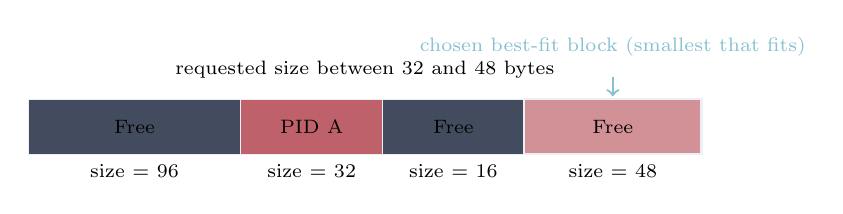
\begin{tikzpicture}[x=0.9cm,y=0.7cm,font=\scriptsize]
  % Block 0: Free (large)
  \draw[fill=Nord2,draw=Nord6] (0,0) rectangle (3,1);
  \node at (1.5,0.5) {Free};
  \node[below] at (1.5,0) {size = 96};

  % Block 1: Allocated
  \draw[fill=Nord11,draw=Nord6] (3,0) rectangle (5,1);
  \node at (4,0.5) {PID A};
  \node[below] at (4,0) {size = 32};

  % Block 2: Free (smaller than needed)
  \draw[fill=Nord2,draw=Nord6] (5,0) rectangle (7,1);
  \node at (6,0.5) {Free};
  \node[below] at (6,0) {size = 16};

  % Block 3: Free (best-fit)
  \draw[fill=Nord11!70,draw=Nord6,thick] (7,0) rectangle (9.5,1);
  \node at (8.25,0.5) {Free};
  \node[below] at (8.25,0) {size = 48};

  % Annotation: request
  \node[above] at (4.75,1.2)
    {requested size between 32 and 48 bytes};

  % Arrow to best-fit
  \draw[->,Nord8,thick] (8.25,1.4) -- (8.25,1.05);
  \node[above,Nord8] at (8.25,1.6)
    {chosen best-fit block (smallest that fits)};
\end{tikzpicture}

\vspace{0.8em}

\begin{itemize}
  \item \texttt{mallocate} scans all blocks: only free blocks are considered.
  \item For each free block, it computes the size and checks if it can fit \texttt{size}.
  \item Among all fitting blocks, it chooses the smallest one.
\end{itemize}

\end{frame}

\begin{frame}[fragile]{Best-Fit Allocation: Commit + Split}
\vspace{-0.5em}
\begin{beamercolorbox}[rounded=true,shadow=true,wd=\textwidth]{block body}
\begin{lstlisting}[
  language=MyC,
  basicstyle=\fontsize{6pt}{7pt}\selectfont\ttfamily,
  aboveskip=0pt,
  belowskip=0pt,
]
  // Reference the chosen best-fit block
  MemoryBlock* best_fit = &MEMBLOCK(index);
  // Save old block bounds
  dword old_start = best_fit->start_addr;
  dword old_end   = best_fit->end_addr;
  // New end address after allocating size bytes
  dword new_end = (old_start + size) - 1;
  // Mark the allocated region as owned by this PID
  best_fit->pid = pid;
  best_fit->is_free = false;
  best_fit->end_addr = new_end;

  // If the block was larger than needed, split the remainder
  if (new_end < old_end) {
    // Shift blocks right to make room for a new free block
    for (int i = MEMORY_TABLE.block_count; i > index + 1; i--) {
      MEMBLOCK(i) = MEMBLOCK(i - 1);
    }
    // Create a new free block with the leftover space
    MEMBLOCK(index + 1).pid = NO_PID;
    MEMBLOCK(index + 1).is_free = true;
    MEMBLOCK(index + 1).start_addr = new_end + 1;
    MEMBLOCK(index + 1).end_addr = old_end;
    MEMORY_TABLE.block_count++;   // Increase block count
  }
  printf("PID %d allocated %d bytes at [%d --> %d]\n",
         pid, size, best_fit->start_addr, best_fit->end_addr);
  return best_fit->start_addr;    // Return the starting address
}
\end{lstlisting}
\end{beamercolorbox}
\end{frame}

\begin{frame}{Best-Fit Allocation: Commit + Split Visualization}
\centering
\scriptsize

\textbf{Before allocation (best-fit block selected)}\\[0.3em]

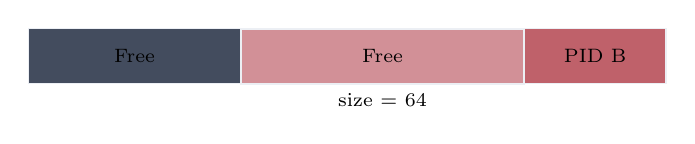
\begin{tikzpicture}[x=0.9cm,y=0.7cm,font=\scriptsize]
  % Free (left)
  \draw[fill=Nord2,draw=Nord6] (0,0) rectangle (3,1);
  \node at (1.5,0.5) {Free};

  % Best-fit free block
  \draw[fill=Nord11!70,draw=Nord6,thick] (3,0) rectangle (7,1);
  \node at (5,0.5) {Free};
  \node[below] at (5,0) {size = 64};

  % Allocated (right)
  \draw[fill=Nord11,draw=Nord6] (7,0) rectangle (9,1);
  \node at (8,0.5) {PID B};
\end{tikzpicture}

\vspace{0.8em}

\textbf{After allocation of \texttt{size} bytes and split}\\[0.3em]

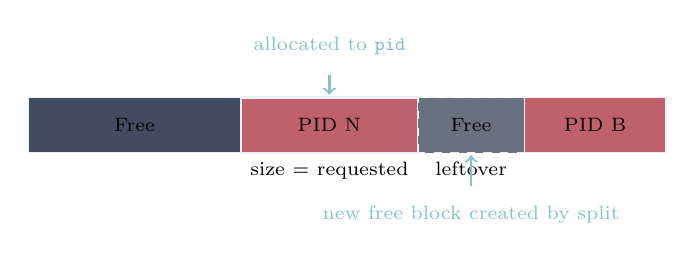
\begin{tikzpicture}[x=0.9cm,y=0.7cm,font=\scriptsize]
  % Free (left)
  \draw[fill=Nord2,draw=Nord6] (0,0) rectangle (3,1);
  \node at (1.5,0.5) {Free};

  % New allocated block for this PID
  \draw[fill=Nord11,draw=Nord6,thick] (3,0) rectangle (5.5,1);
  \node at (4.25,0.5) {PID N};
  \node[below] at (4.25,0) {size = requested};

  % Remainder free block (split portion)
  \draw[fill=Nord2!80,draw=Nord6,dashed] (5.5,0) rectangle (7,1);
  \node at (6.25,0.5) {Free};
  \node[below] at (6.25,0) {leftover};

  % Allocated (right)
  \draw[fill=Nord11,draw=Nord6] (7,0) rectangle (9,1);
  \node at (8,0.5) {PID B};

  % Arrows / explanation
  \draw[->,Nord8,thick] (4.25,1.4) -- (4.25,1.05);
  \node[above,Nord8] at (4.25,1.6)
    {allocated to \texttt{pid}};

  \draw[->,Nord8,thick] (6.25,-0.6) -- (6.25,-0.05);
  \node[below,Nord8] at (6.25,-0.8)
    {new free block created by split};
\end{tikzpicture}

\vspace{0.7em}

\begin{itemize}
  \item The chosen free block is partially consumed by the request.
  \item The used portion becomes an allocated block for this \texttt{pid}.
  \item Any leftover space is turned into a new, smaller free block.
\end{itemize}

\end{frame}



\begin{frame}[fragile]{Freeing Memory: Locate + Mark Free}
\begin{beamercolorbox}[rounded=true,shadow=true,wd=\textwidth]{block body}
\begin{lstlisting}[
  language=MyC,
  basicstyle=\fontsize{7pt}{7pt}\selectfont\ttfamily,
  aboveskip=0pt,
  belowskip=0pt,
]
void liberate(int pid)
{
  int index = 0;

  // Find the memory block owned by this PID
  for (index = 0; index < MEMORY_TABLE.block_count; index++) {
    if (MEMBLOCK(index).pid == pid &&
        !MEMBLOCK(index).is_free) {

      // Mark the block as free
      MEMBLOCK(index).pid = NO_PID;
      MEMBLOCK(index).is_free = true;

      printf("Freed (PID %d) at memory [%d --> %d]\n",
             pid,
             MEMBLOCK(index).start_addr,
             MEMBLOCK(index).end_addr);

      break;
    }
  }

  // PID not found in any allocated block
  if (index == MEMORY_TABLE.block_count)
    return;
\end{lstlisting}
\end{beamercolorbox}
\end{frame}

\begin{frame}[fragile]{Freeing Memory: Coalescing Adjacent Blocks}
\begin{beamercolorbox}[rounded=true,shadow=true,wd=\textwidth]{block body}
\begin{lstlisting}[
  language=MyC,
  basicstyle=\fontsize{5.5pt}{7pt}\selectfont\ttfamily,
  aboveskip=0pt,
  belowskip=0pt,
]
  // Merge with previous free block
  if (index > 0 && MEMBLOCK(index - 1).is_free) {

    // Extend previous block into this one
    MEMBLOCK(index - 1).end_addr = MEMBLOCK(index).end_addr;

    // Shift table left to remove the freed block's entry
    for (int i = index; i < MEMORY_TABLE.block_count - 1; i++) {
      MEMBLOCK(i) = MEMBLOCK(i + 1);
    }

    MEMORY_TABLE.block_count--;
    index--;      // New merged block is now at (index - 1)
  }

  // Merge with next free block
  if (index < MEMORY_TABLE.block_count - 1 &&
      MEMBLOCK(index + 1).is_free) {

    // Extend this block into the next
    MEMBLOCK(index).end_addr = MEMBLOCK(index + 1).end_addr;

    // Shift table left to remove the merged block
    for (int i = index + 1; i < MEMORY_TABLE.block_count - 1; i++) {
      MEMBLOCK(i) = MEMBLOCK(i + 1);
    }

    MEMORY_TABLE.block_count--;
  }
}
\end{lstlisting}
\end{beamercolorbox}
\end{frame}

\begin{frame}{Freeing Memory: Visual Overview}
\centering
\scriptsize

% 1) Before liberate(pid)
\textbf{1. Before \texttt{liberate(pid)}}\\[0.3em]
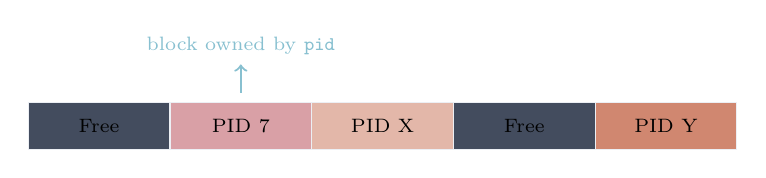
\begin{tikzpicture}[x=0.9cm,y=0.6cm,font=\scriptsize]
  % Free
  \draw[fill=Nord2,draw=Nord6] (0,0) rectangle (2,1)
    node[midway,align=center]{Free};

  % PID 7 (target)
  \draw[fill=Nord11!60,draw=Nord6] (2,0) rectangle (4,1)
    node[midway,align=center]{PID 7};

  % PID X
  \draw[fill=Nord12!60,draw=Nord6] (4,0) rectangle (6,1)
    node[midway,align=center]{PID X};

  % Free
  \draw[fill=Nord2,draw=Nord6] (6,0) rectangle (8,1)
    node[midway,align=center]{Free};

  % PID Y
  \draw[fill=Nord12,draw=Nord6] (8,0) rectangle (10,1)
    node[midway,align=center]{PID Y};

  % Arrow to show block being freed
  \draw[->,Nord8,thick] (3,1.2) -- (3,1.8);
  \node[above,Nord8] at (3,1.8) {block owned by \texttt{pid}};
\end{tikzpicture}

\vspace{0.8em}

% 2) After mark free
\textbf{2. After marking the block free}\\[0.3em]
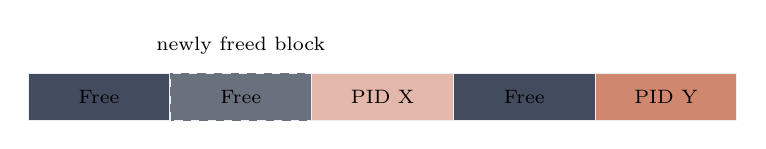
\begin{tikzpicture}[x=0.9cm,y=0.6cm,font=\scriptsize]
  % Free
  \draw[fill=Nord2,draw=Nord6] (0,0) rectangle (2,1)
    node[midway,align=center]{Free};

  % Newly freed block
  \draw[fill=Nord2!80,draw=Nord6,dashed] (2,0) rectangle (4,1)
    node[midway,align=center]{Free};

  % PID X
  \draw[fill=Nord12!60,draw=Nord6] (4,0) rectangle (6,1)
    node[midway,align=center]{PID X};

  % Free
  \draw[fill=Nord2,draw=Nord6] (6,0) rectangle (8,1)
    node[midway,align=center]{Free};

  % PID Y
  \draw[fill=Nord12,draw=Nord6] (8,0) rectangle (10,1)
    node[midway,align=center]{PID Y};

  \node[above] at (3,1.2) {newly freed block};
\end{tikzpicture}

\vspace{0.8em}

% 3) After coalescing
\textbf{3. After coalescing with neighbouring free blocks}\\[0.3em]

\begin{tikzpicture}[x=0.9cm,y=0.6cm,font=\scriptsize]
  % Merged free region (previous + freed + next)
  \draw[fill=Nord2,draw=Nord6] (0,0) rectangle (8,1)
    node[midway,align=center]{Merged Free Region};

  % PID Y
  \draw[fill=Nord12,draw=Nord6] (8,0) rectangle (10,1)
    node[midway,align=center]{PID Y};
\end{tikzpicture}

\end{frame}
%================================================
\section{Module 3: Process Scheduling and Context Switching}
%================================================
\begin{frame}[fragile]{Schedulers}
\vspace{-0.9em}
\begin{beamercolorbox}[rounded=true,shadow=true,wd=\textwidth]{block body}
\begin{lstlisting}[
  language=MyC,
  basicstyle=\fontsize{5pt}{7pt}\selectfont\ttfamily,
  aboveskip=0pt,
  belowskip=0pt,
]
void scheduler(SchedulingAlgorithm algorithm) {
  PerfTimer overall_timer;
  perf_timer_start(&overall_timer);
  const char *algo_name = "Unknown";
  switch (algorithm) {
    case SCHED_FCFS: algo_name = "FCFS"; break;
    case SCHED_ROUND_ROBIN: algo_name = "Round Robin"; break;
    case SCHED_PRIORITY: algo_name = "Priority"; break;
    case SCHED_SRT: algo_name = "SRT"; break;
    case SCHED_HRRN: algo_name = "HRRN"; break;
    case SCHED_SPN: algo_name = "SPN"; break;
    case SCHED_MLFQ: algo_name = "MLFQ"; break;
    default: break;
  }
  g_current_algorithm_id = start_algorithm_tracking(algo_name);
  switch (algorithm) {
    case SCHED_ROUND_ROBIN: roundRobin(); break;
    case SCHED_PRIORITY: priorityBased(); break;
    case SCHED_SRT: shortestRemainingTime(); break;
    case SCHED_HRRN: highestResponseRatioNext(); break;
    case SCHED_FCFS: firstComeFirstServe(); break;
    case SCHED_SPN: shortestProcessNext(); break;
    case SCHED_MLFQ: feedBack(); break;
    default: fprintf(stderr, "Unknown Scheduler Type\n"); break;
  }
  double total_time = perf_timer_end_seconds(&overall_timer);
  if (g_current_algorithm_id >= 0) {
    record_scheduler_time(g_current_algorithm_id, total_time * 1000.0);
    end_algorithm_tracking(g_current_algorithm_id);
    print_algorithm_results(g_current_algorithm_id);
  }
}
\end{lstlisting}
\end{beamercolorbox}
\end{frame}

\begin{frame}[fragile]{Queues}
\begin{beamercolorbox}[rounded=true,shadow=true,wd=\textwidth]{block body}
\begin{lstlisting}[
  language=MyC,
  basicstyle=\fontsize{11pt}{11pt}\selectfont\ttfamily,
  aboveskip=0pt,
  belowskip=0pt,
]
typedef struct {
  int next;
  int capacity;
  Process PCB[];
} Queue;

static Queue* Ready_Queue = NULL;
static Queue* Running_Queue = NULL;
static Queue* Blocked_Queue = NULL;
static Queue* Suspend_Blocked_Queue = NULL;
static Queue* Suspend_Ready_Queue = NULL;
static Queue* New_Queue = NULL;
static Queue* Finished_Queue = NULL;
\end{lstlisting}
\end{beamercolorbox}
\end{frame}

\begin{frame}[fragile]{Round Robin: Context Switching in Our Simulator}
\small

% \textbf{When does a context switch happen?}
% \begin{itemize}
%   \item At the start of each time slice, when we load a new process.
%   \item At the end of the slice, when we save its CPU state and either:
%     \begin{itemize}
%       \item finish the process, or
%       \item preempt it and move it to the back of the ready queue.
%     \end{itemize}
% \end{itemize}

\medskip

\textbf{Switching into a process}
\begin{beamercolorbox}[rounded=true,shadow=true,wd=\textwidth]{block body}
\begin{lstlisting}[
language=MyC,
basicstyle=\fontsize{5.8pt}{7.2pt}
\selectfont\ttfamily]
Process *p = &Ready_Queue->PCB[0];

set_current_process(p->pid);  // Update current PID
THE_CPU = p->cpu_state;       // Restore registers & PC
record_context_switch(g_current_algorithm_id);
\end{lstlisting}
\end{beamercolorbox}

\medskip

\textbf{Switching out of a process}
\begin{beamercolorbox}[rounded=true,shadow=true,wd=\textwidth]{block body}
\begin{lstlisting}[language=MyC,
  basicstyle=\fontsize{5.8pt}{7.2pt}\selectfont\ttfamily]
p->cpu_state = THE_CPU;  // Save registers & PC

if (finished) {
  record_process_completion(p);
  liberate(p->pid);      // Free its memory
  shift_ready_left();    // Remove from ready queue
} else {
  Process tmp = *p;
  shift_ready_left();    // Remove from front
  push_ready_back(tmp);  // Requeue at back (preemption)
}
\end{lstlisting}
\end{beamercolorbox}
\end{frame}

\begin{frame}[fragile]{FCFS: Context Switching in Our Simulator}
\small

\textbf{Switching into a process (once per process)}
\begin{beamercolorbox}[rounded=true,shadow=true,wd=\textwidth]{block body}
\begin{lstlisting}[language=MyC,
  basicstyle=\fontsize{6.8pt}{7.2pt}\selectfont\ttfamily]
Process *p = &Ready_Queue->PCB[0];

if (!p->has_started) {
  p->has_started = true;
  p->start_time = g_system_time;
  p->response_time = g_system_time - p->arrival_time;
}

perf_timer_start(&timer);
set_current_process(p->pid);   // Update current PID
THE_CPU = p->cpu_state;        // Restore registers & PC
record_context_switch(g_current_algorithm_id);
\end{lstlisting}
\end{beamercolorbox}
\end{frame}

\begin{frame}[fragile]{FCFS: Context Switching in Our Simulator}
\textbf{Running non-preemptively until completion}
\begin{beamercolorbox}[rounded=true,shadow=true,wd=\textwidth]{block body}
\begin{lstlisting}[language=MyC,
  basicstyle=\fontsize{6.8pt}{7.2pt}\selectfont\ttfamily]
while (p->burstTime > 0 &&
       THE_CPU.hw_registers[PC] != CPU_HALT) {
  fetch();
  execute();
  p->burstTime--;
  g_system_time++;
}
\end{lstlisting}
\end{beamercolorbox}
\end{frame}

\begin{frame}[fragile]{FCFS: Context Switching in Our Simulator}
\textbf{Switching out of a process (save state + cleanup)}
\begin{beamercolorbox}[rounded=true,shadow=true,wd=\textwidth]{block body}
\begin{lstlisting}[language=MyC,
  basicstyle=\fontsize{6.8pt}{7.2pt}\selectfont\ttfamily]
p->cpu_state = THE_CPU;              // Save final CPU state
double ctx_time = perf_timer_end(&timer);
record_context_switch_time(g_current_algorithm_id, ctx_time);

record_process_completion(p);
liberate(p->pid);                    // Free its memory
shift_ready_left();                  // Next process moves to front
\end{lstlisting}
\end{beamercolorbox}
\end{frame}

\begin{frame}[fragile]{Round Robin: Fetch--Decode--Execute Region}
\begin{beamercolorbox}[rounded=true,shadow=true,wd=\textwidth]{block body}
\begin{lstlisting}[
  language=MyC,
  basicstyle=\fontsize{9pt}{7.2pt}\selectfont\ttfamily,
  aboveskip=0pt,
  belowskip=0pt,
]
int slice = (p->burstTime < QUANTUM) ? p->burstTime : QUANTUM;

// Preemptive time-sliced Fetch--Decode--Execute
for (int i = 0; i < slice; i++) {
  if (THE_CPU.hw_registers[PC] == CPU_HALT)
    break;

  fetch();    // Fetch next instruction into IR
  execute();  // Decode + execute one instruction

  if (p->burstTime > 0) {
    p->burstTime--;   // Consume one unit of CPU burst
    g_system_time++;  // Advance global system time
  }
}
\end{lstlisting}
\end{beamercolorbox}
\end{frame}

\begin{frame}[fragile]{FCFS: Fetch--Decode--Execute Region}


\begin{beamercolorbox}[rounded=true,shadow=true,wd=\textwidth]{block body}
\begin{lstlisting}[
  language=MyC,
  basicstyle=\fontsize{9pt}{7.2pt}\selectfont\ttfamily,
  aboveskip=0pt,
  belowskip=0pt,
]
// Non-preemptive Fetch--Decode--Execute: run until completion
while (p->burstTime > 0 &&
       THE_CPU.hw_registers[PC] != CPU_HALT) {

  fetch();    // Fetch next instruction into IR
  execute();  // Decode + execute one instruction

  p->burstTime--;   // Consume one unit of CPU burst
  g_system_time++;  // Advance global system time
}
\end{lstlisting}
\end{beamercolorbox}


\end{frame}

%================================================
\section{Module 4: Enhanced Interrupt Handling}
%================================================

\begin{frame}[fragile]{Interrupts}
\begin{beamercolorbox}[rounded=true,shadow=true,wd=\textwidth]{block body}
\begin{lstlisting}[
  language=MyC,
  basicstyle=\fontsize{7pt}{7pt}\selectfont\ttfamily,
  aboveskip=0pt, belowskip=0pt,
]
// Types of interrupts in our simulator
typedef enum irq {
  IRQ_TIMER = 0x1,     // Periodic timer interrupt
  IRQ_IO,              // I/O device completed
  IRQ_TRAP,            // Software trap / exception
  IRQ_SYSCALL,         // System call from user process
  IRQ_EOI,             // End Of Interrupt
} IRQ;

// An interrupt request with a priority
typedef struct {
  IRQ irq;
  int priority;
} Interrupt;
\end{lstlisting}
\end{beamercolorbox}
\end{frame}

\begin{frame}[fragile]{Interrupt Vector Table (IVT)}
\begin{beamercolorbox}[rounded=true,shadow=true,wd=\textwidth]{block body}
\begin{lstlisting}[
  language=MyC,
  basicstyle=\fontsize{7pt}{7pt}\selectfont\ttfamily,
  aboveskip=0pt, belowskip=0pt,
]
static isr_t IVT[] = {
  [IRQ_TIMER]   = handle_timer_interrupt,
  [IRQ_IO]      = handle_io_interrupt,
  [IRQ_TRAP]    = handle_trap_interrupt,
  [IRQ_SYSCALL] = handle_syscall_interrupt,
  [IRQ_EOI]     = handle_eoi_interrupt,
};
\end{lstlisting}
\end{beamercolorbox}
\end{frame}


\begin{frame}[fragile]{Interrupt Handler}
\begin{beamercolorbox}[rounded=true,shadow=true,wd=\textwidth]{block body}
\begin{lstlisting}[
  language=MyC,
  basicstyle=\fontsize{7pt}{7pt}\selectfont\ttfamily,
  aboveskip=0pt, belowskip=0pt,
]
static void interrupt_handler(Interrupt intr) {
  // Save the currently running CPU context
  push_cpu_state(THE_CPU);

  // Look up and invoke the correct ISR from the IVT
  if (intr.irq >= IRQ_TIMER && intr.irq <= IRQ_EOI && IVT[intr.irq]) {
    IVT[intr.irq](intr);
  } else {
    fprintf(stderr, "[INTERRUPT ERROR] Unknown IRQ %d\n", intr.irq);
  }

  // Restore CPU context and resume interrupted code
  THE_CPU = pop_cpu_state();
}
\end{lstlisting}
\end{beamercolorbox}
\end{frame}

%================================================
\section{Module 5: Efficiency Analysis of Scheduling Algorithms}
%================================================
\begin{frame}{Avg Response Time Comparison}
\begin{beamercolorbox}[rounded=true,shadow=true,wd=\textwidth]{block body}
    \centering
    \includegraphics[height=0.8\textheight]{../charts/comparison_AvgResponseTime.png}
  \end{beamercolorbox}
\end{frame}

\begin{frame}{Avg Turnaround Time Comparison}
\begin{beamercolorbox}[rounded=true,shadow=true,wd=\textwidth]{block body}
    \centering
    \includegraphics[height=0.8\textheight]{../charts/comparison_AvgTurnaroundTime.png}
  \end{beamercolorbox}
\end{frame}

\begin{frame}{Avg Wait Time Comparison}
\begin{beamercolorbox}[rounded=true,shadow=true,wd=\textwidth]{block body}
    \centering
    \includegraphics[height=0.8\textheight]{../charts/comparison_AvgWaitTime.png}
  \end{beamercolorbox}
\end{frame}

\begin{frame}{Context Switch Comparison}
\begin{beamercolorbox}[rounded=true,shadow=true,wd=\textwidth]{block body}
    \centering
    \includegraphics[height=0.8\textheight]{../charts/comparison_ContextSwitches.png}
  \end{beamercolorbox}
\end{frame}

\begin{frame}{CPU Utilization Comparison}
\begin{beamercolorbox}[rounded=true,shadow=true,wd=\textwidth]{block body}
    \centering
    \includegraphics[height=0.8\textheight]{../charts/comparison_CPUUtilization.png}
  \end{beamercolorbox}
\end{frame}

\begin{frame}{L1 Cache: Hits vs Misses}
  \centering
  \begin{columns}[T,onlytextwidth]
    \column{0.5\textwidth}
\begin{beamercolorbox}[rounded=true,shadow=true,wd=\textwidth]{block body}
      \centering
      \textbf{L1 Cache Hits}\\[0.5em]
      \includegraphics[width=\textwidth,height=0.7\textheight,keepaspectratio]{../charts/comparison_L1Hits.png}
  \end{beamercolorbox}

    \column{0.5\textwidth}
\begin{beamercolorbox}[rounded=true,shadow=true,wd=\textwidth]{block body}
      \centering
      \textbf{L1 Cache Misses}\\[0.5em]
      \includegraphics[width=\textwidth,height=0.7\textheight,keepaspectratio]{../charts/comparison_L1Misses.png}
  \end{beamercolorbox}
  \end{columns}
\end{frame}

\begin{frame}{L2 Cache: Hits vs Misses}
  \centering
  \begin{columns}[T,onlytextwidth]
    \column{0.5\textwidth}
\begin{beamercolorbox}[rounded=true,shadow=true,wd=\textwidth]{block body}
      \centering
      \textbf{L2 Cache Hits}\\[0.5em]
      \includegraphics[width=\textwidth,height=0.7\textheight,keepaspectratio]{../charts/comparison_L2Hits.png}
  \end{beamercolorbox}

    \column{0.5\textwidth}
\begin{beamercolorbox}[rounded=true,shadow=true,wd=\textwidth]{block body}
      \centering
      \textbf{L2 Cache Misses}\\[0.5em]
      \includegraphics[width=\textwidth,height=0.7\textheight,keepaspectratio]{../charts/comparison_L2Misses.png}
  \end{beamercolorbox}
  \end{columns}
\end{frame}

\begin{frame}{Throughput Comparison}
\begin{beamercolorbox}[rounded=true,shadow=true,wd=\textwidth]{block body}
    \centering
    \includegraphics[height=0.8\textheight]{../charts/comparison_Throughput.png}
  \end{beamercolorbox}
\end{frame}


%================================================
\section{Assembler}
%================================================
\begin{frame}{MIPS-1 Assembler}
\small

\textbf{What the assembler does}
\begin{itemize}
  \item Parses \texttt{.text} and \texttt{.data} sections, collecting labels and directives.
  \item Expands pseudo-instructions (e.g., \texttt{li}, \texttt{la}, \texttt{nop}) into real MIPS-1 ops.
  \item Encodes each instruction into its 32-bit machine code format.
  \item Builds a packed data segment (bytes, halfwords, words, strings).
\end{itemize}

\medskip

\textbf{How it integrates with our OS simulator}
\begin{itemize}
  \item Allocates real memory for text/data using \texttt{mallocate()}.
  \item Writes machine code and data directly into the simulated RAM.
  \item Rebases label addresses so instructions like \texttt{j}, \texttt{la}, and \texttt{beq} point to the correct physical addresses.
\end{itemize}

\medskip

\textbf{What it produces}
\begin{itemize}
  \item A complete \texttt{AssembledProgram}: text/data regions, entry point, stack pointer, and symbol table.
  \item Fully loadable, runnable machine code for our CPU's Fetch--Decode--Execute loop.
\end{itemize}

\end{frame}

%================================================
\section{Demonstration}
%================================================

\end{document}
